%priprava posamezne ure
%tukaj zaporedoma napisemo{st. zaporedne ure}{datum}{naslov}{poglavje}{oblika dela}{pripomocki}
\begin{priprava}{}{}{Odvod}{Diferenciali funkcije}{frontalna}{tabla}

Diferenciali funkcije in računanje približnih vrednosti

Primer: Okrog ekvatorja postavimo obroč (polmer je $ x = 6370 $ km). Nato obseg obroča povečamo za 1 m. Izračunaj, ali lahko gre miš skozi luknjo.

nov obseg = $ 40.023.890{,}41 m + 1 m = 40.023.891{,}41 m $

$ r_n = \frac{40.023.891{,}41 m}{2 \pi} = 6370{,}000159 km $

Torej je razlika 15{,}9 cm.


\textcolor{red}{\textbf{Diferencial funkcije:}}

\begin{figure*}[h]
    \centering
    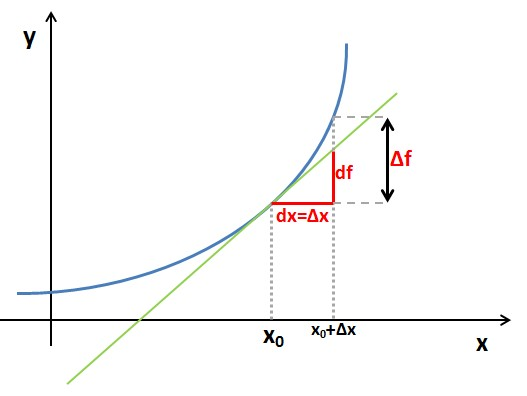
\includegraphics[width=0.5\textwidth]{slike/diferencial.jpg}
\end{figure*}

V limiti diferenčnega kvocienta je sprememba $ \Delta x $ zelo majhna, praktično enaka 0. Označimo jo z $ dx $. Tudi sprememba funkcijske vrednosti $ \Delta f $ je zaradi zveznosti $ f $ ustrezno majhna; označimo jo z $ df $. Tako dobimo
$$ \lim_{\Delta x \to 0} \frac{\Delta f}{\Delta x} = \frac{df}{dx} = f'(x) $$

Izrazimo $ df = f'(x) dx $ in to poimenujemo \textbf{diferencial}. Diferencial elahko uporabljamo pri približnem računanju funkcijskih vrednosti za funkcije, kjer je računanje prave funkcijske vrednosti prezapleteno.

Primer: Izračunaj približno vrednost $ \sqrt{4{,}01} $.

Torej imamo $ f(x) = \sqrt{x} $. Poznamo $ f(4) = 2 $ in $ f'(4) = \frac{1}{4} $. Uporabimo formulo \textcolor{red}{$ f(x_0 + h) \doteq f(x_0) + df(x_0) $} \didopomba{ali jo izpeljemo ali samo povemo}.

$ f(4 + 0{,}01) = f(4) + f'(4) \cdot 0{,}01 = 2 + 0{,}025 = 2{,}025 $.

Vrednost s kalkulatorjem: 2{,}002498439.

\vaje{
Vaje:
\begin{itemize}
    \item 
\end{itemize}
}
    
\end{priprava}